\begin{figure}[htb]
  \begin{center}
    \resizebox{\textwidth}{!}{
      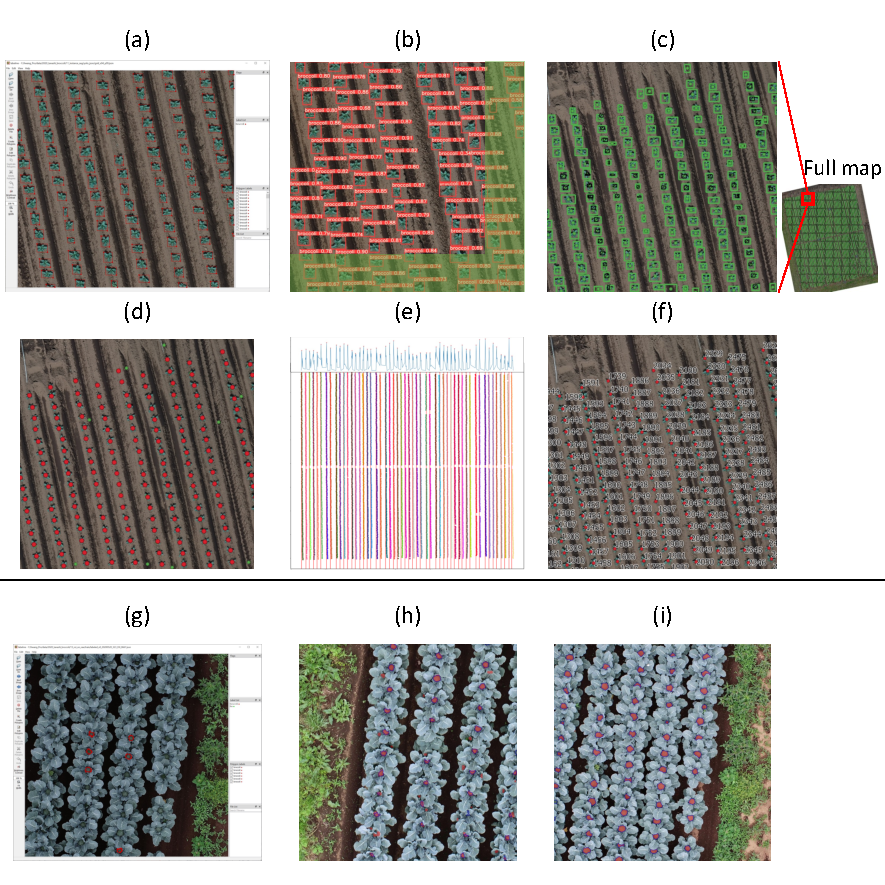
\includegraphics{figures/bro/Fig.S1_deep_learning_demo.pdf}
    }
  \end{center}
  \caption[Examples of 2020 broccoli seedling position detection and head segmentation by interactive annotation]{
    Examples of 2020 broccoli seedling position detection (a-f) and head segmentation by interactive annotation (g-i). 
    (a) One annotated training data by LabelMe. 
    (b) YOLO v5 detected results; the green part is the buffer zone to avoid the broken broccoli plants at the edge. 
    (c) Duplicate detection in buffer zone removed by the non-maximum suppression (NMS) algorithm. Black shows removed duplicate detection, green shows those that were retained, and green dots are the center points as the broccoli position. 
    (d) Red dots show the manually adjusted positions by QGIS. 
    (e) Ridge detection by identifying the peak of points distribution. 
    (f) Automatic placing of plant ID along the ridge. 
    (g) Startup training data annotation made by LabelMe; only a few annotations were required. 
    (h) After the first iteration. The red polygons are the segmentation results (as auxiliary annotations) trained by the startup data and the blue polygons are manually adjusted according to the previous results. 
    (i) After the fourth iteration, almost no manual adjustment was required in this case.
  }
  \label{fig:bros1}
\end{figure}